\documentclass[aspectratio=169,14pt]{beamer}
\usetheme{beamerthemeTalentSprint}
\usepackage[utf8]{inputenc}
\usepackage{graphics}
\usepackage{ragged2e}
\usepackage{amsfonts}
\usepackage{xcolor}
\usepackage{tcolorbox}
\usepackage{setspace}
\definecolor{swe}{rgb}{0.19, 0.73, 0.56}
\title[Decision Trees]{Decision Trees}

\begin{document}

{ \1
\begin{frame} \vspace{35pt}
%	\title[Decision Trees]{Decision Trees}
	\subtitle{Classification Algorithms}
	\maketitle
	\end{frame}
	}

% Frame: 2
\begin{frame}{Decision Trees}
\begin{itemize}
\item Most popular tool - Kaggle
\item Easy to understand 
\item Like a flow chart
\item if-else rules
\end{itemize}
\end{frame}

% Frame: 3
\begin{frame}[fragile]{Decision Trees}
\begin{columns}
\column{0.5\textwidth}
\hspace{8cm} 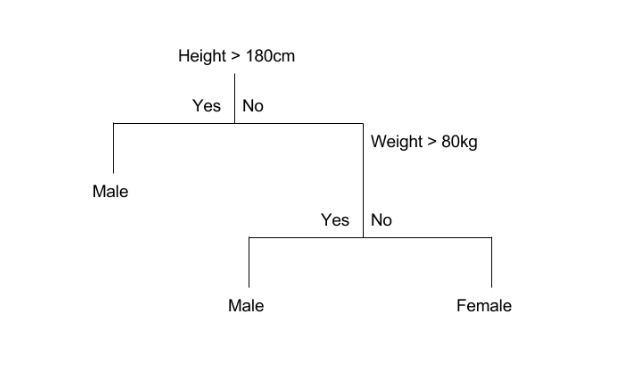
\includegraphics[width=8cm,height=5.5cm]{Images/dtree1_3.png}
\column{0.5\textwidth}
%\begin{tcolorbox}[width=6.5cm, height=3.5cm, sharp corners, left=0pt,right=0pt,colback={pink!60!white}]
%\scriptsize
%	\begin{verbatim}
%		if(Height > 180cm)
%			return Male
%		else
%			if(Weight > 80kg)
%				return Male
%			else
%				return Female
%	\end{verbatim}
%\end{tcolorbox}
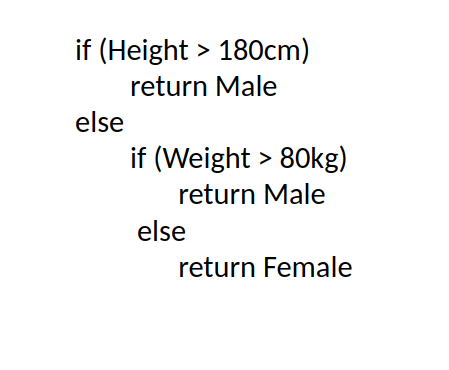
\includegraphics[width=8cm,height=5.5cm]{Images/dtree1_3a.png}
\end{columns}
\end{frame}

% Frame: 4
\begin{frame}{Pseudo Code for Decision Tree}
	\begin{tcolorbox}[width=14cm,boxrule=0pt, sharp corners,left=0pt,right=0pt,colback={blue!5!white}]
\begin{itemize}
\item Place the \alert{best} features of the dataset at the root of the tree
\item Split the training set into \alert{subsets}
\item Repeat step 1 and step 2 on each subset until you find \alert{leaf nodes} in all the branches of the tree
\end{itemize}
\end{tcolorbox}
\end{frame}




% Frame: 5
\begin{frame}{Decision Tree}
\begin{itemize}
\item Splitting Criterion 1: Based on Weight?
\item Splitting Criterion 2: Based on Height?
\item Who chose the order?
\item On what basis? 
\end{itemize}
\end{frame}


% Frame: 6
\begin{frame}{Experiment}

\begin{itemize}
\item \href{https://drive.google.com/file/d/1_WWveEZ3Os0rCU0M1Dghrvi5INsaHxyd/view?usp=sharing}{Demo\_DT\_Fruits\_data}
	\begin{itemize}
		\item Dataset : Fruits 
		\item Objective : To classify data using Decision tree classifier
	\end{itemize}
\end{itemize}
\end{frame}


% Frame: 7
\begin{frame}{Decision Tree with Depth 2}
\centering
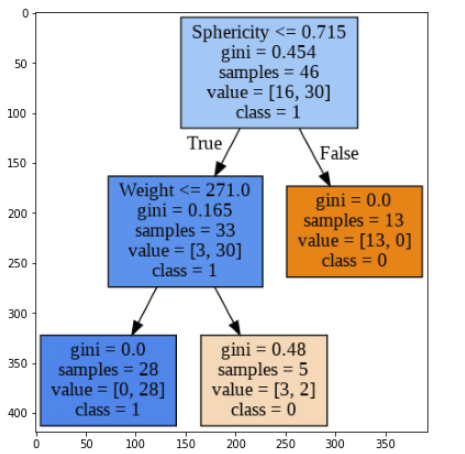
\includegraphics[width=0.4\textwidth, height=0.7\textheight]{Images/dtree2.png}
\end{frame}

% Frame: 8
\begin{frame}{Decision Tree with Depth 2}
\begin{columns}
%	\column{0.1\textwidth}
\column{0.5\textwidth}
	\begin{flushright}
		\vspace{-1cm}
		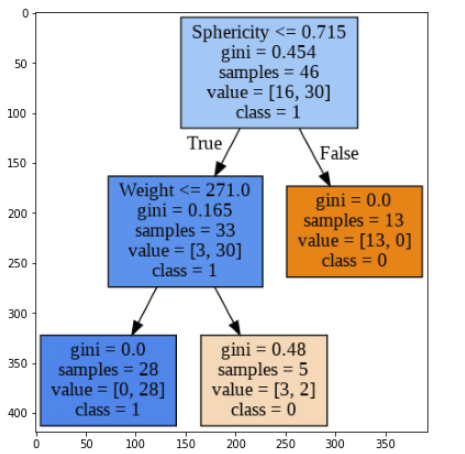
\includegraphics[width=6cm,  height=5.5cm]{Images/dtree2.png}
	\end{flushright}
\column{0.4\textwidth}
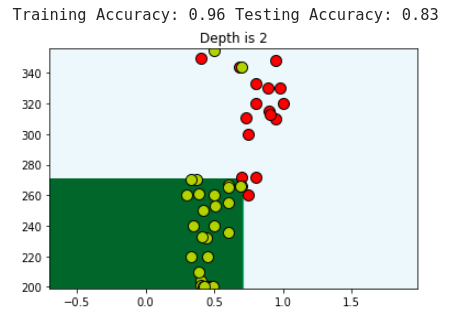
\includegraphics[width=7.5cm, height=5cm]{Images/depth2.png}\\

	\column{0.1\textwidth}
\end{columns}
\end{frame}

% Frame: 9
\begin{frame}{Decision Tree with Depth 3}
\centering
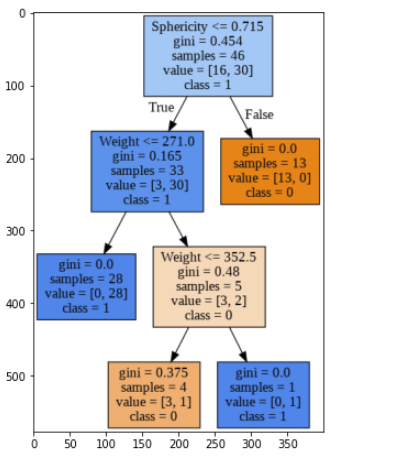
\includegraphics[width=7cm, height=6cm]{Images/dtree3.png}
\end{frame}

% Frame: 10
\begin{frame}{Decision Tree with Depth 3}
\begin{columns}
\column{8cm}
\centering
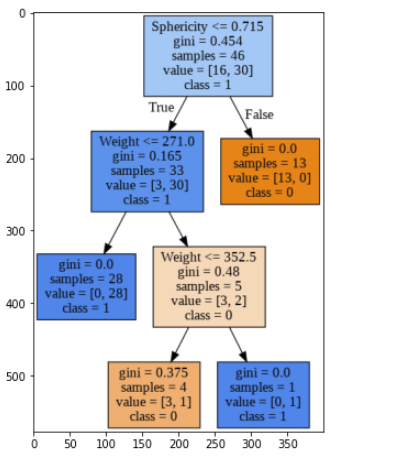
\includegraphics[width=6cm, height=6cm]{Images/dtree3.png}
\column{8cm}
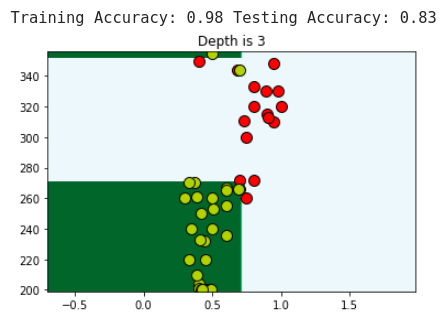
\includegraphics[width=7cm, height=4.5cm]{Images/depth3.png} \\

\end{columns}
\end{frame}

% Frame: 11
\begin{frame}{Summary}
\begin{itemize}
\item \alert{Decision Tree:}
	\begin{itemize}
		\item  Simple Human understandable solution
	\end{itemize}
\item \alert{Training:} Finding the best tree
	\begin{itemize}
		\item  Best criteria
		\item  Best value to test the criteria against
		\item  Best sequence of criteria
	\end{itemize}
\item \alert{Testing:} Use criteria obtained in training stage to classify
\end{itemize}
\end{frame}


% Frame: 13
{\1
\begin{frame}
	\title{Thanks!!}
	\subtitle{Questions?}
	\maketitle
\end{frame}
}

\end{document}


